\bookchapter{第四十二章：大模型全景与API实战}

\chapterintro{前面几章讲的都是“怎么和 AI 协作”，本章解决一个更基础的问题：“用哪个 AI？怎么用？”2026 年 8 月的大模型格局已经极其丰富——国际有 GPT、Claude、Gemini 三强争霸，国内有 DeepSeek、通义千问、GLM、Kimi、豆包百花齐放。每个模型都有自己的性格和特长：选对了事半功倍，选错了事倍功半。本章不仅带你认识这些模型，还会教你如何通过 API 将它们接入自己的应用，以及如何根据自己的需求选择合适的 Token Plan（用量套餐）。}

\booksection{一、国际主流大模型：三强格局}

2026 年 8 月的国际大模型市场，形成了 OpenAI（GPT 系列）、Anthropic（Claude 系列）、Google（Gemini 系列）三强鼎立的格局。每家都有自己鲜明的特色——咱们一个一个认识。

\booksubsection{OpenAI GPT-5.6 系列：全能均衡的六边形战士}

OpenAI 是大模型浪潮的开启者，GPT 系列至今仍是全球使用最广泛的模型。2026 年 7 月发布的 GPT-5.6 系列采用三档定位策略：旗舰款 GPT-5.6 Sol 面向高端推理需求，均衡款 GPT-5.6 Terra 面向日常开发，轻量款 GPT-5.6 Luna 面向高并发低成本场景。三款模型共享 105 万 Token 的上下文窗口，都支持图像输入、函数调用和结构化输出。

\begin{center}
\begin{tabularx}{\linewidth}{|X|X|X|X|X|}
\hline
\textbf{型号} & \textbf{定位} & \textbf{输入(/百万Token)} & \textbf{输出(/百万Token)} & \textbf{上下文窗口} \tabularnewline
\hline
GPT-5.6 Sol & 旗舰推理 & US\$5.00 (约36元) & US\$30.00 (约217元) & 105万Token \tabularnewline
GPT-5.6 Terra & 均衡日常 & US\$2.50 (约18元) & US\$15.00 (约109元) & 105万Token \tabularnewline
GPT-5.6 Luna & 轻量低成本 & US\$1.00 (约7元) & US\$6.00 (约44元) & 105万Token \tabularnewline
\hline
\end{tabularx}
\end{center}

\begin{center}\small\color{gray}OpenAI GPT-5.6 系列定价（2026 年 8 月）\end{center}

GPT 系列的核心优势在于“均衡”——推理、编程、写作、多模态，没有明显短板。加上 OpenAI 庞大的插件生态和开发者社区，适配文档和工具链最为完善。对于“不知道选什么”的场景，GPT 是“闭眼选都不会错”的默认答案。但它的短板是：国内访问需要特殊网络，中文表达偶尔有“翻译腔”，API 价格处于中高水平。

\textbf{好消息}\par

OpenAI 在 2026 年 8 月宣布免费用户默认模型升级为 GPT-5.6 Luna，并开放无限量文本聊天。这意味着你可以零成本体验 GPT 的基础能力，只有在需要更强推理或 API 调用时才需要付费。

\booksubsection{Anthropic Claude 系列：编程与严谨的天花板}

如果说 GPT 是全能选手，那 Claude 就是编程领域的“天花板”。Anthropic 的 Claude 系列在 SWE-bench（软件工程基准测试）上长期断层领先，代码生成质量和工程级项目落地能力业界第一。更难得的是，Claude 的幻觉率（生成虚假信息的概率）全网最低，仅约 1\%——这使它特别适合学术、法务等高精度场景。

Claude 的另一个杀手锏是超长上下文：支持 100 万 Token 的上下文窗口，能一次性“读完”几百页的合同或整个代码库不漏细节。这在代码重构、长文档分析等场景中几乎无可替代。Claude Code 作为终端 AI 编程工具，到 2026 年中期年化收入已达 25 亿美元——这是 Claude 编程能力最受认可的证据。

\begin{center}
\begin{tabularx}{\linewidth}{|X|X|X|X|X|}
\hline
\textbf{型号} & \textbf{定位} & \textbf{输入(/百万Token)} & \textbf{输出(/百万Token)} & \textbf{上下文窗口} \tabularnewline
\hline
Claude Fable 5 & 旗舰款 & US\$10.00 (约72元) & US\$50.00 (约362元) & 100万Token \tabularnewline
Claude Opus 4.8 & 专业款 & US\$5.00 (约36元) & US\$25.00 (约181元) & 100万Token \tabularnewline
Claude Sonnet 5 & 性价比款 & US\$2.00 (约14元) & US\$10.00 (约72元) & 100万Token \tabularnewline
\hline
\end{tabularx}
\end{center}

\begin{center}\small\color{gray}Anthropic Claude 系列定价（2026 年 8 月，Sonnet 5 为优惠价）\end{center}

Claude 的短板是价格——Fable 5 的输出价格是所有模型中最高的，每百万 Token 要 50 美元。多模态能力（图像、视频理解）也相对较弱。对于预算有限的个人开发者，Sonnet 5 在优惠期内的性价比非常突出。

\booksubsection{Google Gemini 系列：多模态的王者}

Google 的 Gemini 系列在 2026 年已迭代至 3.1 Pro 版本。Gemini 的最大杀手锏是原生多模态——图文解析精准、OCR 表格识别无误、视频帧提取高效，还支持音视频深度解析。它与 Google 生态（搜索、邮箱、云服务）深度绑定，在实时信息检索和跨模态理解上表现突出。Gemini 还支持\textbf{200 万 Token}的超长上下文输入，是目前上下文窗口最大的模型。

Gemini 的定位是“科学推理和多模态场景的首选”。如果你的项目涉及大量图像分析、视频理解或科学计算，Gemini 几乎没有对手。但它在纯文本代码生成上略逊于 Claude，中文表达也不如国产模型自然。

\begin{center}
\begin{tabularx}{\linewidth}{|X|X|X|X|}
\hline
\textbf{对比项} & \textbf{GPT-5.6} & \textbf{Claude Fable 5} & \textbf{Gemini 3.1 Pro} \tabularnewline
\hline
综合得分 & 94.8 & 95.0 & 92.1 \tabularnewline
编程能力(SWE-bench) & 74.9\% & 64.3\% (Pro) & 中等 \tabularnewline
上下文窗口 & 105万Token & 100万Token & 200万Token \tabularnewline
多模态能力 & 均衡 & 较弱 & 最强 \tabularnewline
幻觉率 & 较低 & 最低(约1\%) & 较低 \tabularnewline
国内可用性 & 需特殊网络 & 需特殊网络 & 需特殊网络 \tabularnewline
API 生态 & 最完善 & 成长中 & Google 生态绑定 \tabularnewline
\hline
\end{tabularx}
\end{center}

\begin{center}\small\color{gray}国际三大模型横向对比（2026 年 8 月）\end{center}

\begin{tcbwarn}{注意：国内使用的现实门槛}
对于国内开发者来说，GPT、Claude、Gemini 的核心障碍是网络访问。虽然可以通过 Azure 代理、API 聚合平台等方式间接使用，但稳定性和合规性需要自行评估。如果你的项目对数据安全有严格要求，建议优先考虑国产模型。

\end{tcbwarn}

\booksection{二、国产主流大模型：百花齐放}

2026 年的国产大模型已经从“追赶者”变成了“并跑者”，在某些领域甚至实现了“领跑”。与 2023 年“套壳”争议不同，2026 年的国产旗舰模型在逻辑推理、代码生成、中文理解等方面已经与国际一线模型旗鼓相当，差距缩减到 5\% 以内。更重要的是，国产模型在中文场景、价格成本和合规部署上有不可替代的优势。

\booksubsection{DeepSeek V4：性价比之王}

DeepSeek（深度求索）是国产大模型中现象级的存在。2025 年初，DeepSeek-V3 以“比 GPT 便宜十分之一但能力相当”的定位震撼市场，被业内称为“通用 AI 大模型斩杀线”——\textbf{比它便宜的没它好用，比它贵的没它量大管饱}。到 2026 年 8 月，DeepSeek V4-Pro 正式版发布：1.6 万亿参数 MoE 架构，激活约 49B，支持 100 万无损上下文，代码性价比被广泛认为是全球天花板。

DeepSeek V4 在 Agent 能力上实现了大幅跃升——DeepSWE 基准从 12.8 跳至 62.7（+390\%），NL2Repo 从 38.5 升至 61.5。API 新增了 Responses API 与 Anthropic API 双协议支持，已兼容 Codex 和 Claude Code 等主流编程工具。这意味着你可以用 DeepSeek 的 API 替代 Claude 的 API，在 Claude Code 中使用——\textbf{成本降低数倍，体验几乎一致}。

\begin{center}
\begin{tabularx}{\linewidth}{|X|X|X|X|X|}
\hline
\textbf{型号} & \textbf{定位} & \textbf{输入(/百万Token)} & \textbf{输出(/百万Token)} & \textbf{上下文窗口} \tabularnewline
\hline
DeepSeek V4 Pro & 旗舰推理 & 3元 (约US\$0.43) & 6元 (约US\$0.87) & 100万Token \tabularnewline
DeepSeek V4 Flash & 轻量快速 & 1元 (约US\$0.14) & 2元 (约US\$0.28) & 100万Token \tabularnewline
\hline
\end{tabularx}
\end{center}

\begin{center}\small\color{gray}DeepSeek V4 系列定价（2026 年 8 月，促销价）\end{center}

价格对比：同样 100 万 Token 的输入 + 100 万 Token 的输出，DeepSeek V4 Flash 花费约 0.42 美元，GPT-5.6 Sol 花费约 35 美元，Claude Fable 5 花费约 60 美元。\textbf{差距高达 80-140 倍}。

\textbf{避坑提醒：DeepSeek 要涨价了}\par

DeepSeek 官方已于 2026 年 8 月 6 日公告“计划近期大幅上调 API 定价”，促销价可能不会持续太久。部分媒体传闻涨幅可能达 30 倍，截至 8 月 14 日官方尚未公布最终调价方案。此外，DeepSeek V4 正式版引入了\textbf{峰谷定价机制}——高峰时段调用价格直接翻倍。建议关注官方公告获取最新定价。

\booksubsection{通义千问 Qwen3.7 Max：阿里云的企业级选择}

阿里云的通义千问（Qwen）系列依托阿里云生态，在企业级部署上有天然优势。2026 年 7 月的 Qwen3.7 Max 是当前旗舰：235B 参数稠密模型，256K 原生上下文，可扩展至 1M。Qwen 的核心优势在于：开源生态成熟（从 7B 到 235B 全系列开源）、中文场景理解精准、与阿里云基础设施深度集成。

\begin{center}
\begin{tabularx}{\linewidth}{|X|X|X|}
\hline
\textbf{型号} & \textbf{输出价格(/百万Token)} & \textbf{适用场景} \tabularnewline
\hline
qwen-turbo & 0.6元 & 极简问答、文本分类、高并发 \tabularnewline
qwen-long & 2.0元 & 10M 超长上下文处理 \tabularnewline
qwen3.7-flash & 7.2元 & 通用对话、内容生成 \tabularnewline
qwen3.7-plus & 12.0元 & 多模态（图片+视频）、中文创作 \tabularnewline
qwen3.7-max & 36.0元 & 旗舰中文能力、复杂任务 \tabularnewline
\hline
\end{tabularx}
\end{center}

\begin{center}\small\color{gray}通义千问 Qwen 系列阶梯定价（2026 年 8 月）\end{center}

Qwen 的定价采用阶梯策略——从极低成本的 qwen-turbo（输出 0.6 元/百万 Token）到旗舰 qwen3.7-max（输出 36 元/百万 Token），覆盖从轻量问答到复杂推理的全场景需求。对于已经在使用阿里云的企业，Qwen 是最顺手的集成选择。

\booksubsection{智谱 GLM-5.1：国产 SWE-bench 第一}

智谱 AI 的 GLM 系列在 2026 年表现亮眼。GLM-5.1 在 SWE-bench 上拿下\textbf{国产第一}的成绩：744B MoE 稠密混合架构，支持 100 万上下文。它的特点是中文语义理解精准，支持国内合规私有化部署——这对数据安全要求高的金融、政务场景非常重要。GLM-5.1 的定价为输入 6 元、输出 24 元每百万 Token，处于国产模型中游水平。

\booksubsection{Kimi K3：超长文本之王}

月之暗面的 Kimi 系列以超长文本处理能力著称。2026 年 7 月发布的 Kimi K3 拥有 2.8 万亿参数规模，在多项复杂任务评测中进入全球第一梯队。Kimi 的核心场景是长代码库分析和长文档检索增强——它能处理整本书的文本或整个项目的代码，在“大海捞针”式检索任务中表现卓越。Kimi 的定价相对较高（输出约 12-20 元/百万 Token），但在长文本场景的性价比无人能及。

\booksubsection{豆包 Doubao：字节跳动的全能选手}

字节跳动的豆包系列在 2026 年表现稳定。Doubao Seed 2.1 Pro 是火山引擎旗舰模型，256K 上下文，在实测中综合发挥稳定，中文场景体验突出。豆包的优势在于：\textbf{注册即送大量免费 Token}，火山引擎生态集成完善，定价处于国内最低梯队之一。对于想要快速体验 AI 编程的初学者，豆包是零门槛的入门选择。

\begin{center}
\begin{tabularx}{\linewidth}{|X|X|X|X|X|X|}
\hline
\textbf{对比项} & \textbf{DeepSeek V4} & \textbf{Qwen3.7 Max} & \textbf{GLM-5.1} & \textbf{Kimi K3} & \textbf{豆包 2.1 Pro} \tabularnewline
\hline
综合得分 & 87.5 & 89.7 & 90.5 & 88+ & 85+ \tabularnewline
编程能力 & 极强 & 强 & 国产SWE第一 & 强 & 中上 \tabularnewline
中文理解 & 优秀 & 优秀 & 精准 & 优秀 & 优秀 \tabularnewline
上下文窗口 & 100万 & 256K-1M & 100万 & 超长 & 256K \tabularnewline
输出价格(元/M) & 6 & 36 & 24 & 12-20 & 30 \tabularnewline
开源 & MIT协议 & 全系列开源 & 部分开源 & 闭源 & 闭源 \tabularnewline
私有化部署 & 支持 & 支持 & 支持 & 不支持 & 不支持 \tabularnewline
\hline
\end{tabularx}
\end{center}

\begin{center}\small\color{gray}国产五大模型横向对比（2026 年 8 月）\end{center}

一个重要的趋势是：\textbf{国产模型与 GPT/Claude 的“代差感”已经消失}。在逻辑推理和数学竞赛上，国产旗舰与 GPT-5 的分差基本在个位数。在系统化架构思维和复杂工程推理上，Claude 仍然领先——它能给出更有“灵气”的架构方案，而国产模型有时显得“教条”。但在中文场景、成本控制和合规部署上，国产模型有压倒性优势。

\begin{center}
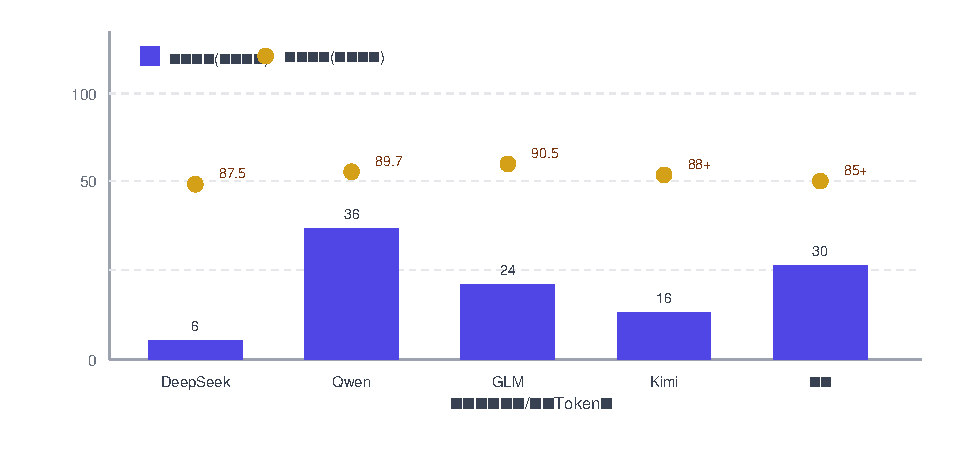
\includegraphics[width=0.92\linewidth]{figures/fig-di-si-shi-er-zhang-1}
\\[2pt]\small 图 4：五款模型的价格与性能对比（价格越低越好，得分越高越好）
\end{center}

\booksection{三、模型选择决策框架}

了解了各模型的特点后，如何为自己的项目选模型？这里送你一套\textbf{“四问决策法”}——回答四个问题，就能锁定最适合你的模型。

你的项目在国内还是国际部署？

国内 选国产模型

|

国际 可选海外模型

核心任务是编程还是其他？

编程 Claude 或 DeepSeek

|

其他 继续判断

需要超长上下文(>50万Token)？

需要 Gemini 或 Kimi

|

不需要 继续判断

预算敏感吗？

敏感 DeepSeek 或 Qwen-turbo

|

不敏感 GPT-5.6 或 Claude

\begin{center}\small\color{gray}图 5：大模型选择四问决策法\end{center}

\begin{tcbinfo}{小贴士：组合策略}
这个决策法不是教条——很多场景需要组合使用多个模型。一个常见的组合策略：用 DeepSeek 或 Qwen 做日常开发（成本低、中文好），用 Claude 做关键架构设计（推理强、幻觉低），用 Gemini 做多模态分析（图像视频处理）。按需切换模型，而不是“一个模型用到死”。

\end{tcbinfo}

\booksection{四、API 调用入门：从零开始接入大模型}

很多 AI 编程教程只教你怎么用对话界面，但真正的“AI 编程”——让你的应用调用大模型——需要通过 API。API（Application Programming Interface，应用程序编程接口）是程序之间的通信协议。通过 API，\textbf{你的代码可以像调用一个函数一样，调用大模型的能力}。

\booksubsection{什么是 Token}

在了解 API 之前，必须先理解 “Token” 这个概念。Token 是大模型计费的基本单位，可以理解为\textbf{“AI 的阅读和写作单位”}。一个 Token 大约对应：英文中 0.75 个单词（4 个字符），中文中 0.5-1 个汉字。一段 1000 字的中文文本，大约消耗 1500-2000 个 Token。

Token 不是字数，也不是字符数。大模型使用专门的分词器（Tokenizer）将文本切分成 Token。同一个词在不同模型中的 Token 数量可能不同——比如“人工智能”在 GPT 中可能是 3 个 Token，在 DeepSeek 中可能是 2 个。大多数模型的 API 会返回实际消耗的 Token 数量，你可以在 API 响应中查看。

\begin{tcbinfo}{Token 成本快速估算}
100 万字中文约等于 150 万 Token。用 DeepSeek V4 Flash 处理 100 万字输入 + 100 万字输出，成本约 0.42 美元（约 3 元人民币）；用 Claude Fable 5 处理同样的量，成本约 60 美元（约 434 元人民币）。\textbf{这就是为什么模型选择直接影响你的项目成本}。

\end{tcbinfo}

\booksubsection{获取 API Key}

使用大模型 API 的第一步是获取 API Key——一串用于身份验证的密钥。每个模型提供商都有自己的 API 平台，你需要注册账号并创建 API Key。以下是主流模型的 API 平台入口和获取流程：

\begin{center}
\begin{tabularx}{\linewidth}{|X|X|X|X|}
\hline
\textbf{模型} & \textbf{API 平台} & \textbf{获取流程} & \textbf{免费额度} \tabularnewline
\hline
DeepSeek & platform.deepseek.com & 注册 实名认证 创建 API Key & 新用户赠送额度 \tabularnewline
通义千问 & bailian.aliyun.com（百炼平台） & 阿里云账号登录 开通服务 创建 Key & 新用户免费试用 \tabularnewline
智谱GLM & open.bigmodel.cn & 注册 实名认证 创建 API Key & 新用户赠送额度 \tabularnewline
Kimi & platform.moonshot.cn & 注册 实名认证 创建 API Key & 有限免费额度 \tabularnewline
豆包 & volcengine.com（火山引擎） & 注册 开通方舟 创建 API Key & 注册送大量 Token \tabularnewline
OpenAI GPT & platform.openai.com & 注册 绑定信用卡 创建 API Key & 无免费额度(需付费) \tabularnewline
Anthropic Claude & console.anthropic.com & 注册 绑卡 创建 API Key & 新用户少量额度 \tabularnewline
\hline
\end{tabularx}
\end{center}

\begin{center}\small\color{gray}主流模型 API 平台及 Key 获取方式（2026 年 8 月）\end{center}

\textbf{安全提示：API Key = 钱包密码}\par

API Key 等同于你的钱包密码——任何拿到 Key 的人都可以用你的额度调用模型。因此：\textbf{永远不要把 API Key 写在代码中}（用环境变量管理）；永远不要把含 Key 的代码提交到公开的 Git 仓库；永远不要在社交媒体分享含 Key 的截图。如果 Key 泄露了，立即在平台上删除并重新创建。

\booksubsection{第一次 API 调用}

获取 API Key 后，你可以用任何编程语言调用大模型 API。以下用 Python 演示一个最简单的调用——向 DeepSeek 发送一条消息并获取回复。

\begin{lstlisting}[language=Python]
# 安装SDK：pip install openai
# DeepSeek兼容OpenAI SDK格式，可以直接用
from openai import OpenAI
import os

# 1. 创建客户端（API Key从环境变量读取）
client = OpenAI(
    api_key=os.environ.get("DEEPSEEK_API_KEY"),
    base_url="https://api.deepseek.com"
)

# 2. 发送请求
response = client.chat.completions.create(
    model="deepseek-chat",  # 指定模型
    messages=[
        {"role": "system", "content": "你是一个Python编程助手。"},
        {"role": "user", "content": "写一个快速排序函数。"}
    ]
)

# 3. 获取回复
print(response.choices[0].message.content)

# 4. 查看Token消耗
print(f"输入Token: {response.usage.prompt_tokens}")
print(f"输出Token: {response.usage.completion_tokens}")
print(f"总Token: {response.usage.total_tokens}")
\end{lstlisting}

这段代码的核心逻辑是：\textbf{创建客户端（携带 API Key 和模型地址） 构造消息列表（system 设定角色，user 是用户输入） 发送请求 获取回复}。这个模式几乎适用于所有兼容 OpenAI 格式的模型——只需要更换 api\_key 和 base\_url 就能切换模型。这就是为什么很多国产模型选择兼容 OpenAI SDK 格式：开发者只需改两行代码就能切换模型，迁移成本极低。

以下是切换到其他模型的代码差异——注意只需要改两行：

\begin{lstlisting}[language=Python]
# DeepSeek
client = OpenAI(
    api_key=os.environ.get("DEEPSEEK_API_KEY"),
    base_url="https://api.deepseek.com"
)
# model="deepseek-chat"

# 通义千问（百炼平台）
client = OpenAI(
    api_key=os.environ.get("DASHSCOPE_API_KEY"),
    base_url="https://dashscope.aliyuncs.com/compatible-mode/v1"
)
# model="qwen-plus"

# 智谱GLM
client = OpenAI(
    api_key=os.environ.get("GLM_API_KEY"),
    base_url="https://open.bigmodel.cn/api/paas/v4"
)
# model="glm-4"

# OpenAI GPT
client = OpenAI(
    api_key=os.environ.get("OPENAI_API_KEY"),
    # base_url使用默认值即可
)
# model="gpt-5.6-terra"
\end{lstlisting}

\booksubsection{流式响应处理}

在实际应用中，你通常不希望等 AI 写完所有内容才一次性显示——那会让用户等太久。流式响应（Streaming）可以让你在 AI 生成的同时逐字显示，大幅提升用户体验。就像打字机一样，字一个一个蹦出来，用户的感觉是完全不同的。

\begin{lstlisting}[language=Python]
# 流式响应：逐字输出
stream = client.chat.completions.create(
    model="deepseek-chat",
    messages=[
        {"role": "user", "content": "写一个Python的冒泡排序教程"}
    ],
    stream=True  # 开启流式响应
)

# 逐块接收并打印
for chunk in stream:
    if chunk.choices[0].delta.content is not None:
        print(chunk.choices[0].delta.content, end="", flush=True)
# 输出会像打字机一样逐字显示
\end{lstlisting}

\booksection{五、Token Plan 购买指南}

大多数模型提供商有两种计费方式：按量计费（Pay-as-you-go）和套餐订阅（Token Plan / Subscription）。理解这两种方式的区别，能帮你大幅降低使用成本。

\booksubsection{按量计费 vs 套餐订阅}

\begin{center}
\begin{tabularx}{\linewidth}{|X|X|X|}
\hline
\textbf{维度} & \textbf{按量计费(Pay-as-you-go)} & \textbf{套餐订阅(Subscription)} \tabularnewline
\hline
计费方式 & 用多少Token付多少钱 & 预付固定费用，获得额度 \tabularnewline
适合场景 & 使用量不稳定、偶尔调用 & 使用量稳定、高频调用 \tabularnewline
价格优势 & 标准价 & 比按量低20\%-50\% \tabularnewline
灵活性 & 随时可用，无需承诺 & 需要预付，额度过期可能作废 \tabularnewline
超额处理 & 自动按量计费 & 超出额度后转为按量计费 \tabularnewline
代表平台 & 各模型官方API平台 & OpenAI Plus/Pro, Claude Pro, Cursor Pro \tabularnewline
\hline
\end{tabularx}
\end{center}

\begin{center}\small\color{gray}两种计费方式的对比\end{center}

对于初学者，建议\textbf{从按量计费开始}——不需要预付费用，用多少花多少。当你的月使用量稳定在一个水平后（比如每月超过 50 元），再考虑切换到套餐订阅以获得更低单价。

\booksubsection{主流订阅套餐一览}

\begin{center}
\begin{tabularx}{\linewidth}{|X|X|X|X|}
\hline
\textbf{套餐} & \textbf{月费} & \textbf{包含内容} & \textbf{适合人群} \tabularnewline
\hline
ChatGPT Free & 免费 & GPT-5.6 Luna 无限文本对话 & 零基础体验 \tabularnewline
ChatGPT Plus & US\$20/月 & GPT-5.6 Sol、图像生成、数据分析、插件访问 & 中度使用者 \tabularnewline
ChatGPT Pro & US\$200/月 & 无限制使用所有模型、优先访问新功能 & 重度专业用户 \tabularnewline
Claude Free & 免费 & 有限次数Claude对话 & 零基础体验 \tabularnewline
Claude Pro & US\$20/月 & 无限制Claude使用、优先访问新模型 & 编程开发者 \tabularnewline
Cursor Free & 免费 & 有限次数AI补全和对话 & 初学者体验 \tabularnewline
Cursor Pro & US\$20/月 & 无限AI补全、500次/月高级请求 & 日常开发者 \tabularnewline
Cursor Business & US\$40/月/人 & 团队协作、管理后台、隐私模式 & 团队使用 \tabularnewline
\hline
\end{tabularx}
\end{center}

\begin{center}\small\color{gray}主流 AI 工具订阅套餐（2026 年 8 月）\end{center}

国内模型的订阅方案略有不同。DeepSeek 主要按量计费，没有月度订阅套餐——你充值后按实际使用量扣费。通义千问在百炼平台提供预付费资源包（购买一定量的 Token 额度，享受折扣价）。豆包在火山引擎上也有类似的预付费方案。对于国内开发者，最经济的组合通常是：\textbf{DeepSeek 按量计费（日常开发）+ 豆包免费额度（体验测试）}。

\booksubsection{API 聚合平台}

如果你需要同时使用多个模型，API 聚合平台是一个省心的选择。聚合平台提供一个统一的 API Key，你就能调用全球几十种模型，无需在每个平台分别注册。

\begin{center}
\begin{tabularx}{\linewidth}{|X|X|X|X|}
\hline
\textbf{平台} & \textbf{特点} & \textbf{价格优势} & \textbf{适合场景} \tabularnewline
\hline
OpenRouter (openrouter.ai) & 海外聚合平台，一个Key调用全球模型 & 价格透明，支持实时比价 & 需要灵活切换多个海外模型 \tabularnewline
SiliconFlow (siliconflow.cn) & 国内聚合平台，提供多种国产模型API & 比官方低20\%-30\% & 国内开发者，多模型比价 \tabularnewline
Azure OpenAI (微软代理) & 微软Azure代理的OpenAI API & Batch API可打5折 & 企业级OpenAI调用，大批量异步任务 \tabularnewline
百度千帆 (qianfan.baidubce.com) & 百度AI云平台，提供文心等模型 & 新用户赠送额度 & 百度生态用户 \tabularnewline
\hline
\end{tabularx}
\end{center}

\begin{center}\small\color{gray}主流 API 聚合平台（2026 年 8 月）\end{center}

\textbf{避坑提醒：别买“共享 Key”}\par

不要在淘宝、闲鱼等平台购买所谓的“共享 API Key”——这些 Key 通常来路不明，可能随时被封号，还有数据泄露风险。始终通过官方平台或正规聚合平台获取 API Key。

\booksubsection{成本优化策略}

选对模型只是第一步，如何“用得省钱”同样重要。以下是几个经过实践验证的成本优化策略：

\begin{enumerate}
  \item \textbf{善用缓存命中}。很多模型提供"缓存"功能——当你的请求中包含之前已经处理过的内容（如系统提示词），这部分只按极低价格计费。DeepSeek 的缓存命中价格仅为普通价格的 1/60。把固定的系统提示放在消息列表开头，可以最大化缓存命中。
  \item \textbf{分级路由}——用便宜模型处理简单任务，贵模型处理复杂任务。比如用 DeepSeek V4 Flash 做文本分类（输出 2 元/百万 Token），用 Claude 做架构设计（输出 181 元/百万 Token）。一个项目里 80\% 的调用可以用便宜模型。
  \item \textbf{限制输出长度}。API 按输出 Token 计费，输出越长越贵。在不需要长篇大论的场景中，设置 max\_tokens 参数限制输出长度，避免 AI"废话太多"。
  \item \textbf{使用 Batch API 处理非实时任务}。如果你有大量不需要即时响应的任务（如批量数据标注、文档摘要），使用 Batch API 可以享受 50\% 折扣。OpenAI 和 Azure 都提供这个功能。
  \item \textbf{监控 Token 用量}。大多数 API 平台提供用量统计面板。定期查看用量分布，找出消耗 Token 最多的调用，针对性优化。一个小小的 Prompt 调整（比如把"请详细解释"改成"请用 3 句话解释"）可能节省 50\% 的 Token。
\end{enumerate}

\begin{center}
\begin{tabularx}{\linewidth}{|X|X|X|X|}
\hline
\textbf{优化策略} & \textbf{节省幅度} & \textbf{实施难度} & \textbf{说明} \tabularnewline
\hline
缓存命中 & 最高98\% & 低 & 把固定内容放在消息开头 \tabularnewline
分级路由 & 50\%-80\% & 中 & 简单任务用便宜模型 \tabularnewline
限制输出长度 & 30\%-60\% & 低 & 设置max\_tokens参数 \tabularnewline
Batch API & 50\% & 低 & 非实时任务用批处理 \tabularnewline
Prompt优化 & 20\%-50\% & 中 & 精简Prompt，减少冗余 \tabularnewline
\hline
\end{tabularx}
\end{center}

\begin{center}\small\color{gray}成本优化策略及效果（2026 年 8 月）\end{center}

\booksection{六、实战：在项目中接入大模型 API}

让我们用一个完整的实战来结束本章——创建一个\textbf{“AI 摘要生成器”}：用户输入一段长文本，调用大模型 API 生成摘要。这个实战会展示 API 调用的完整流程：环境配置、API 调用、错误处理、成本控制。

\begin{lstlisting}[language=Python]
# ai_summarizer.py - AI摘要生成器
import os
from openai import OpenAI

# 1. 配置（API Key从环境变量读取，绝不硬编码）
client = OpenAI(
    api_key=os.environ.get("DEEPSEEK_API_KEY"),
    base_url="https://api.deepseek.com"
)

def summarize(text: str, max_length: int = 200) -> dict:
    """生成文本摘要

    Args:
        text: 要摘要的原文
        max_length: 摘要最大长度（Token数）

    Returns:
        dict: 包含摘要和Token消耗信息
    """
    try:
        response = client.chat.completions.create(
            model="deepseek-chat",
            messages=[
                {
                    "role": "system",
                    "content": "你是一个摘要生成器。"
                               "请用简洁的中文总结用户提供的文本。"
                               "摘要不超过3句话。"
                },
                {
                    "role": "user",
                    "content": f"请摘要以下文本:\n\n{text}"
                }
            ],
            max_tokens=max_length,  # 限制输出长度
            temperature=0.3  # 低温度=更稳定
        )

        return {
            "success": True,
            "summary": response.choices[0].message.content,
            "input_tokens": response.usage.prompt_tokens,
            "output_tokens": response.usage.completion_tokens,
            "total_tokens": response.usage.total_tokens
        }

    except Exception as e:
        return {
            "success": False,
            "error": str(e)
        }

# 2. 使用示例
if __name__ == "__main__":
    long_text = """
    （粘贴一段长文本...）
    """

    result = summarize(long_text)

    if result["success"]:
        print(f"摘要: {result['summary']}")
        print(f"消耗Token: {result['total_tokens']}")
        # 估算成本：DeepSeek V4 Flash
        cost = result['total_tokens'] * 0.000004  # 约0.4分/千Token
        print(f"预估成本: {cost:.4f}元")
    else:
        print(f"出错了: {result['error']}")
\end{lstlisting}

这段代码体现了 API 调用的几个最佳实践：API Key 通过环境变量读取，绝不硬编码在代码中；函数有清晰的文档和类型提示；设置了 max\_tokens 限制输出长度；temperature 设为低值（0.3）以获得更稳定的输出；有完整的错误处理；返回 Token 消耗信息用于成本追踪。当你用 AI 来写这段代码时，可以告诉它这些要求——它完全有能力帮你实现。

本章的最终启示：模型是"弹药"，方法论是"战术"。选对弹药能让战斗更顺利，但没有好的战术，再好的弹药也打不赢仗。了解了各模型的特点和 API 使用方法后，你就有了一个充足的"弹药库"——但怎么打这场仗，还是要靠前几章学到的思维方法论。

\begin{tcbpractice}{来动手：跑通你的第一次 API 调用}
注册一个国产模型平台（推荐 DeepSeek 或智谱，都送新用户额度），创建 API Key，把它写进系统环境变量（而不是代码里！），然后运行上面“第一次 API 调用”的代码。看到 AI 的回复打印出来的那一刻，你就跨过了“用 AI”和“造 AI 应用”之间的分界线。

\end{tcbpractice}

\begin{tcbsummary}{本章小结}
\begin{itemize}
  \item 国际三强：GPT-5.6（均衡全能）、Claude（编程天花板+幻觉率仅1\%）、Gemini（多模态之王+200万上下文）
  \item 国产五强：DeepSeek V4（性价比之王，注意涨价公告）、Qwen3.7（企业级）、GLM-5.1（SWE国产第一）、Kimi K3（超长文本）、豆包（免费入门）
  \item 四问决策法：部署地点？编程还是其他？超长上下文？预算敏感？
  \item Token 是计费单位：中文 1 字约 1.5-2 Token；100万字约150万Token
  \item API Key = 钱包密码：环境变量管理，绝不硬编码、不上传Git
  \item 国产模型普遍兼容 OpenAI SDK：换模型只需改 api\_key 和 base\_url 两行
  \item 省钱五招：缓存命中、分级路由、限制输出、Batch API、监控用量
\end{itemize}

\end{tcbsummary}
